\section{Trajectory outcomes and the advective comparison}

Trajectories use immutable source snapshots. Failed and bounded outcomes remain terminal; no failed state is restarted or relabeled. Crosses in the plots mark the last reported diagnostic, which can precede the actual failure time below. Table times are coordinate times; multiply by three to obtain $t/M$. The numerator guard is sampled approximately every $0.025$ coordinate-time units, so a reported stop is not an exact onset time.

\begin{center}\small\begin{tabular}{llrrl}\toprule

Candidate / test & $N$ & Target $t$ & Accepted $t$ & Outcome\\\midrule

Direct pulse & 65 & 0.1 & 0.1 & completed\\

Direct pulse & 65 & 1 & 0.223256 & failed\\

Direct puncture & 257 & 0.2 & 0.15 & failed\\

Adaptive pulse & 65 & 0.1 & 0.1 & completed\\

Adaptive pulse & 65 & 1 & 0.223256 & failed\\

Adaptive puncture & 257 & 0.2 & 0.15 & failed\\

Direct pulse & 129 & 1 & 0.224125 & failed\\

Adaptive pulse & 129 & 1 & 0.224125 & failed\\

\bottomrule\end{tabular}\end{center}

All 6 failed segments stop on the scri numerator guard. Their last accepted times and resolutions are retained in the table.

No candidate with a failed regular-center gate is promoted to a long puncture evolution. Consequently the $100M$ comparison, final-$20M$ drift fit for a new candidate, and a statement of improved late-time settling are unavailable. This is a failed qualification of the tested boundary implementation, not a measured puncture failure at $100M$ or a rejection of every discretization of the bulk equations.

The advective $N=257$ trajectory completes $100.0002M$. Its final relative horizon-mass error is $-2.563\times10^{-5}$, with peak sampled drift $1.655\times10^{-4}$. Its compact horizon radius changes from 0.062924 to 0.170409. The least-squares slope over $80.025$--$100.0002M$ is $9.306\times10^{-4}$ per unit $t/M$, with fit RMS $1.769\times10^{-4}$. Its final exterior mixed field-rate RMS is $9.073\times10^{-2}$. This surviving reference has not reached a stationary coordinate state by this diagnostic.

For the direct control puncture test, the last accepted time is $0.45M$. Peak sampled relative horizon-mass drift is $2.511\times10^{-9}$ and the last reported absolute relative mass error is $2.921\times10^{-9}$. There are 7 exact shared diagnostic times with the old history. The complete histories retain their native sample spacing; no unequal-time profile is used as a refinement comparison.

For the adaptive reference puncture test, the last accepted time is $0.45M$. Peak sampled relative horizon-mass drift is $2.509\times10^{-9}$ and the last reported absolute relative mass error is $2.919\times10^{-9}$. There are 7 exact shared diagnostic times with the old history. The complete histories retain their native sample spacing; no unequal-time profile is used as a refinement comparison.

At the latest exact shared diagnostic time, $t/M=0.45$, the direct control has the following finite-resolution comparison:

\begin{center}\small\begin{tabular}{lrrr}\toprule

Metric & New & Advective & New / old\\\midrule

Exterior H RMS & $1.424\times10^{-3}$ & $1.452\times10^{-3}$ & 0.9808\\

Exterior M RMS & $2.544\times10^{-2}$ & $2.811\times10^{-3}$ & 9.05\\

Exterior Theta RMS & $1.514\times10^{-5}$ & $5.025\times10^{-6}$ & 3.013\\

Exterior Z RMS & $1.619\times10^{-2}$ & $1.180\times10^{-4}$ & 137.2\\

\bottomrule\end{tabular}\end{center}

The compact horizon radii at this same time are 0.06478981 (new) and 0.06552123 (advective). This short comparison cannot establish a reduced late-time drift rate.

At the latest exact shared diagnostic time, $t/M=0.45$, the adaptive reference has the following finite-resolution comparison:

\begin{center}\small\begin{tabular}{lrrr}\toprule

Metric & New & Advective & New / old\\\midrule

Exterior H RMS & $1.425\times10^{-3}$ & $1.452\times10^{-3}$ & 0.981\\

Exterior M RMS & $2.440\times10^{-2}$ & $2.811\times10^{-3}$ & 8.681\\

Exterior Theta RMS & $1.471\times10^{-5}$ & $5.025\times10^{-6}$ & 2.927\\

Exterior Z RMS & $1.554\times10^{-2}$ & $1.180\times10^{-4}$ & 131.7\\

\bottomrule\end{tabular}\end{center}

The compact horizon radii at this same time are 0.06479176 (new) and 0.06552123 (advective). This short comparison cannot establish a reduced late-time drift rate.

\clearpage\subsection{Diagnostic plots}

\begin{figure}[htbp]\centering

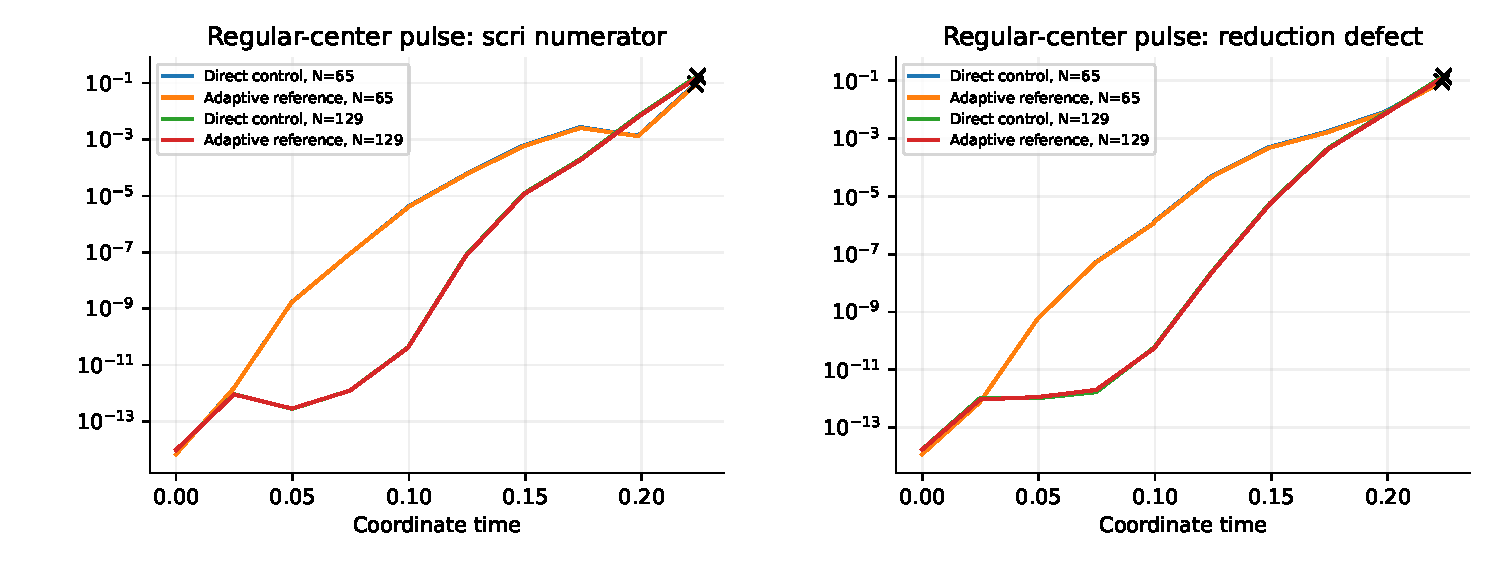
\includegraphics[width=\linewidth]{figures/pulse-gates.pdf}

\caption{Regular-center pulse gates, in coordinate time. The numerator and derivative-reduction defects expose boundary growth separately from exact nullness.}\end{figure}

\begin{figure}[htbp]\centering

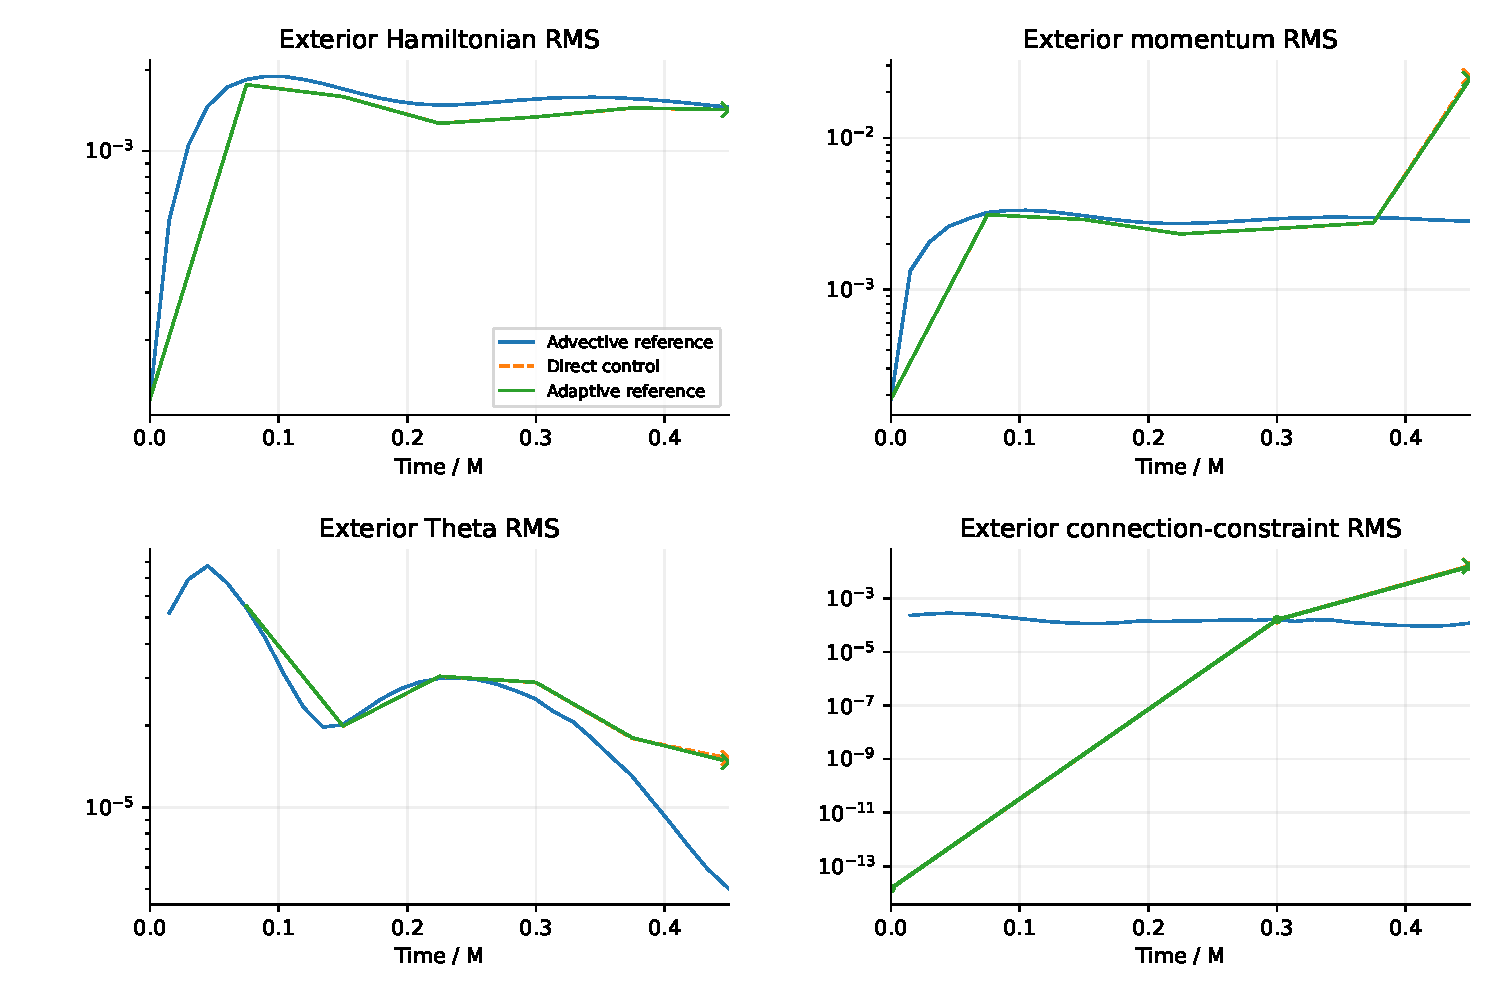
\includegraphics[width=\linewidth]{figures/exterior-constraints.pdf}

\caption{Apparent-horizon-exterior RMS Hamiltonian, momentum, Theta, and connection constraints. The primary Z curves use independent metric finite differences on saved profiles and terminal states; the other three diagnostics agree with the independently recomputed values there. Norms are normalized over exterior radial weights. Zero values are omitted only on logarithmic axes.}\end{figure}

\begin{figure}[htbp]\centering

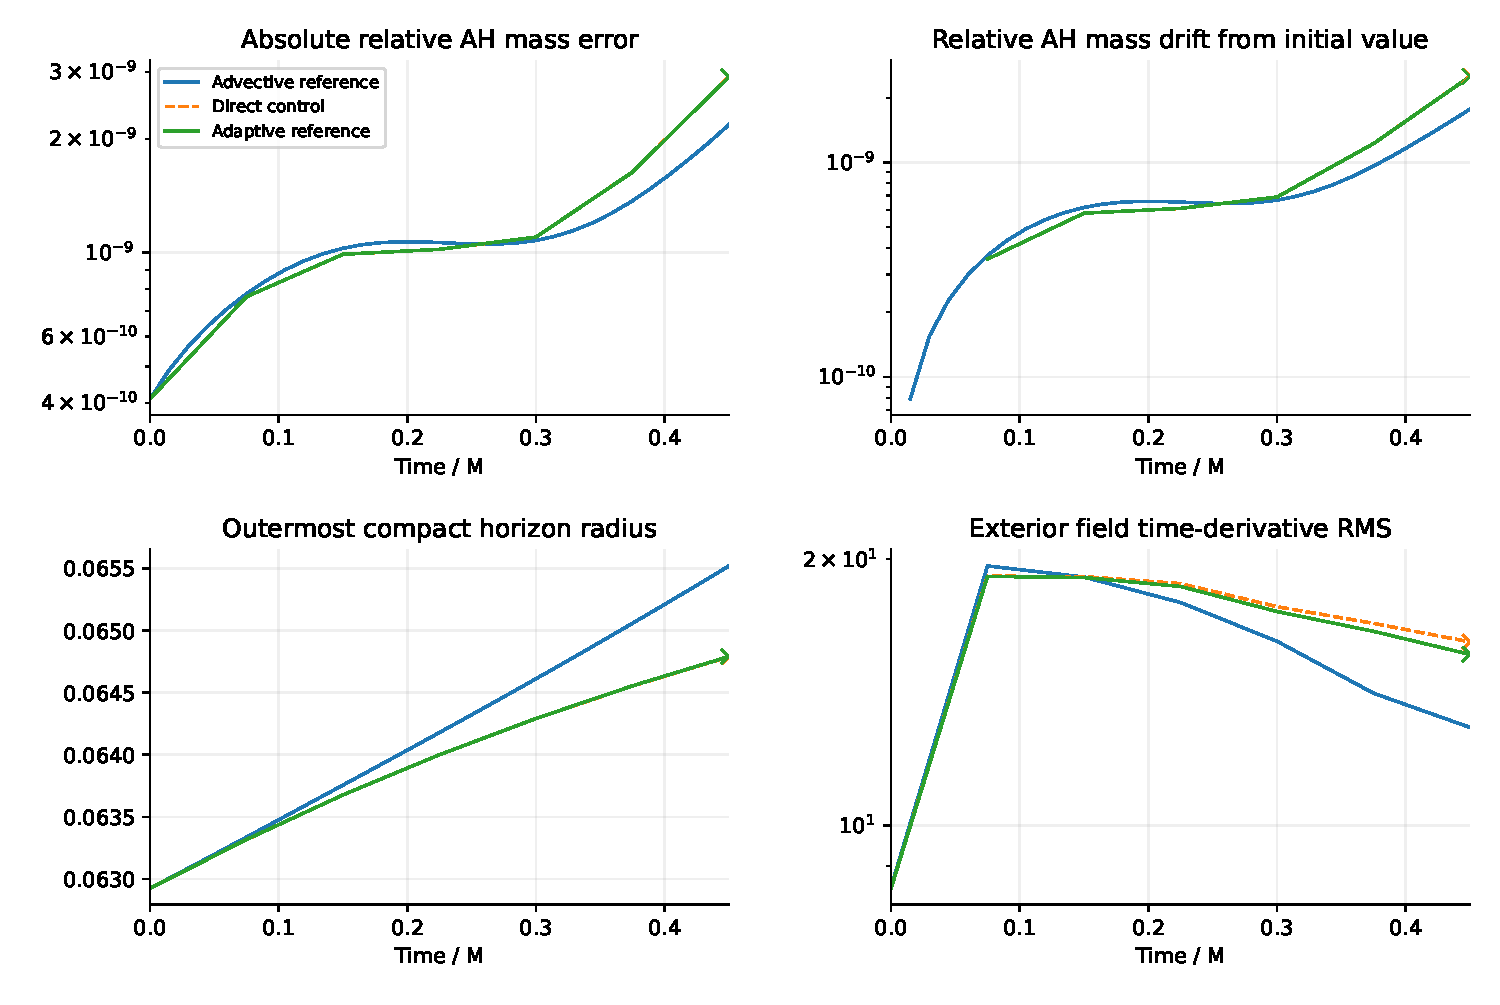
\includegraphics[width=\linewidth]{figures/mass-horizon-settling.pdf}

\caption{Outermost-horizon mass error, drift from each numerical initial mass, compact horizon radius, and candidate field-rate RMS. The time window shows the actual short candidate evidence; it does not imply a late-time comparison. Reference field rates at the short common times come from read-only diagnostics on the exactly recovered sampling replay; its 100M value is reported separately.}\end{figure}

\begin{figure}[htbp]\centering

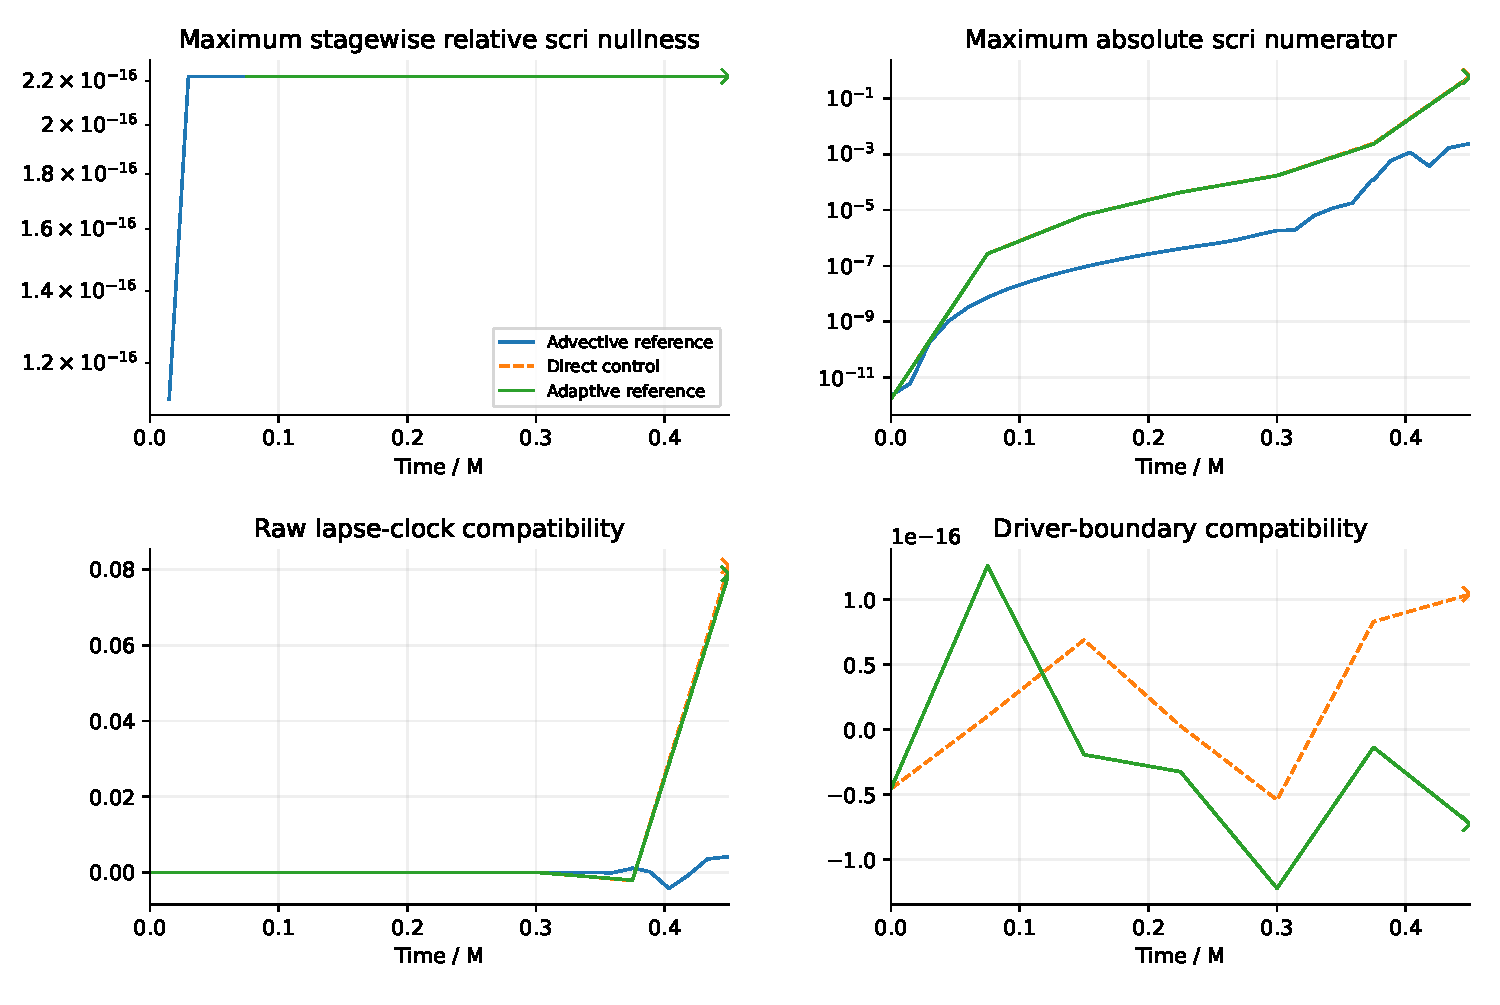
\includegraphics[width=\linewidth]{figures/boundary-health.pdf}

\caption{Maximum stagewise relative nullness, current numerator residual, raw lapse-clock compatibility, and the new driver compatibility residual. Roundoff gauge identities can coexist with growing regularity errors.}\end{figure}

\begin{figure}[htbp]\centering

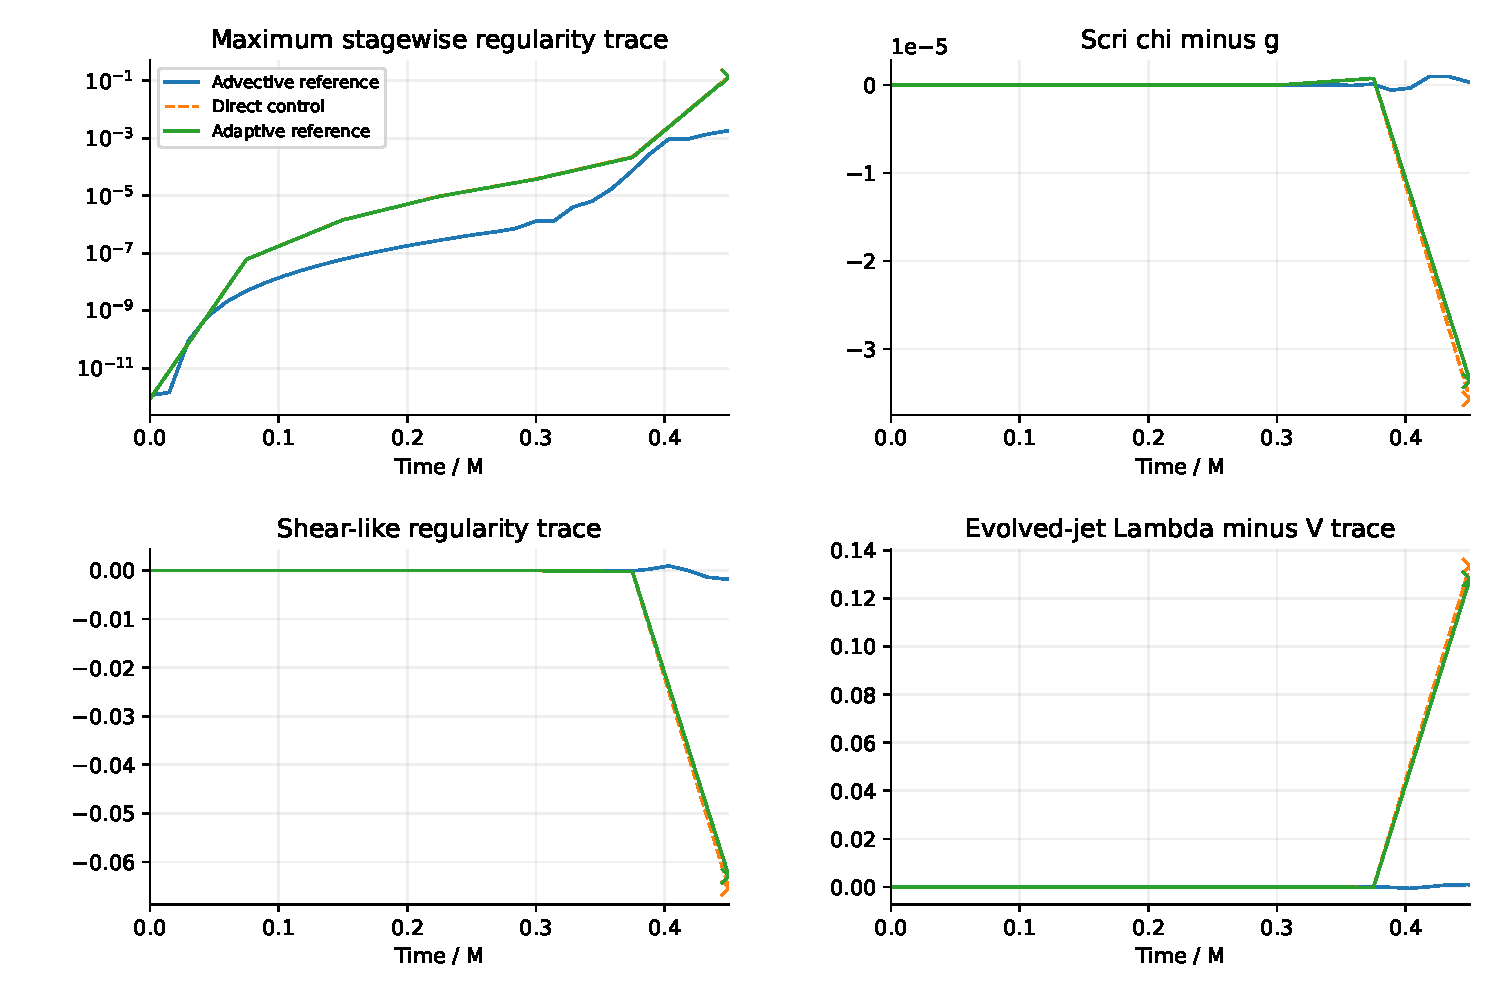
\includegraphics[width=\linewidth]{figures/regularity-traces.pdf}

\caption{Approximate regularity traces, distinct from exact nullness. These use the evolved boundary jet, whose inconsistency with metric reconstruction is quantified separately.}\end{figure}

\begin{figure}[htbp]\centering

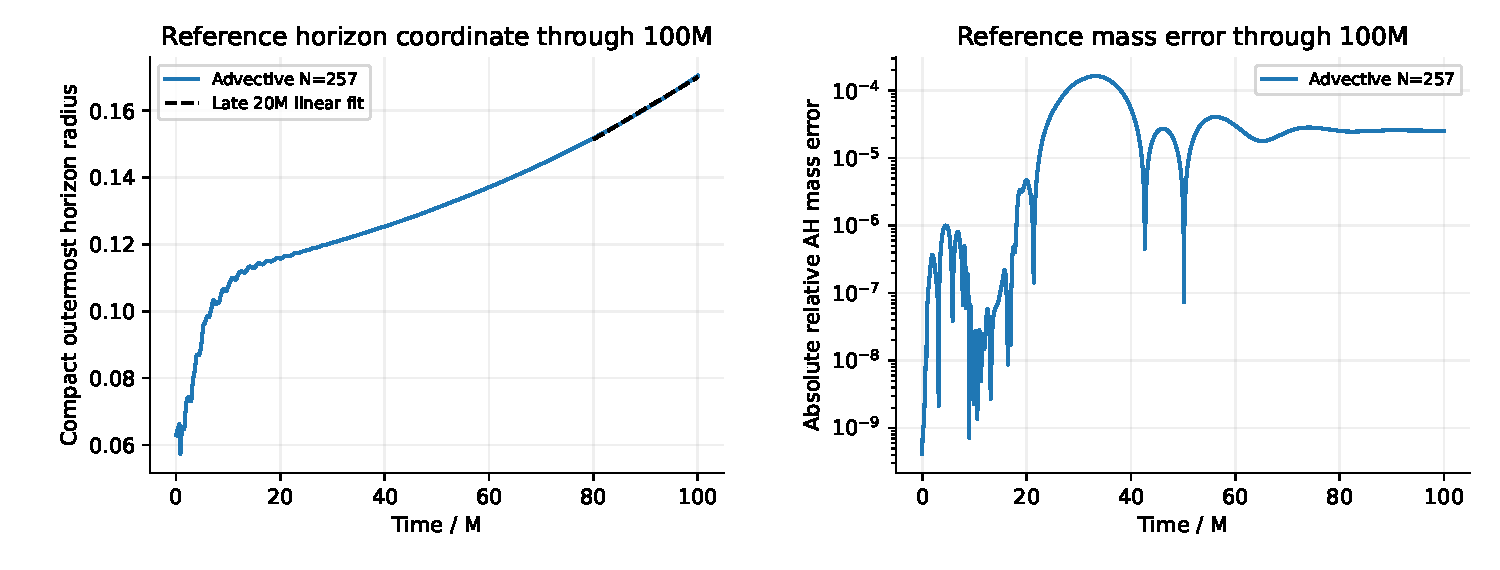
\includegraphics[width=\linewidth]{figures/advective-duration-context.pdf}

\caption{The preserved advective duration context. The late horizon-coordinate fit uses the final $20M$; no new candidate reaches this interval. Short matched new profiles and histories are shown separately.}\end{figure}

\begin{figure}[htbp]\centering

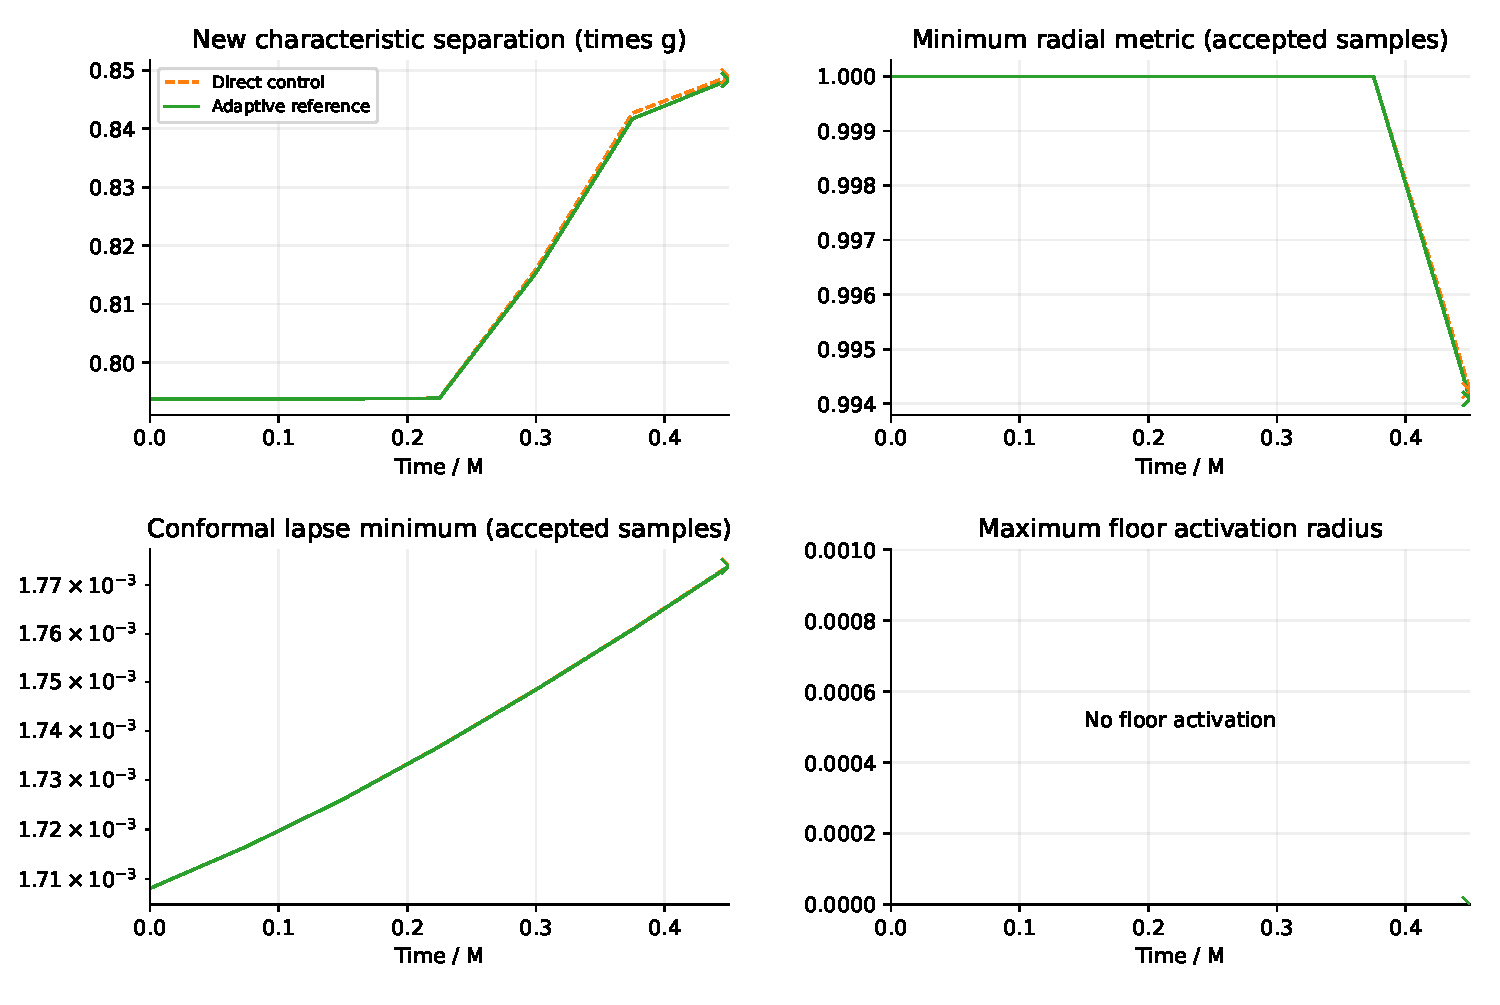
\includegraphics[width=\linewidth]{figures/gauge-positivity-floor.pdf}

\caption{New sufficient characteristic-separation margin, geometry minima at accepted diagnostic samples, and maximum stage floor radius. The old advective gap has a different definition and is not superposed.}\end{figure}

\begin{figure}[htbp]\centering

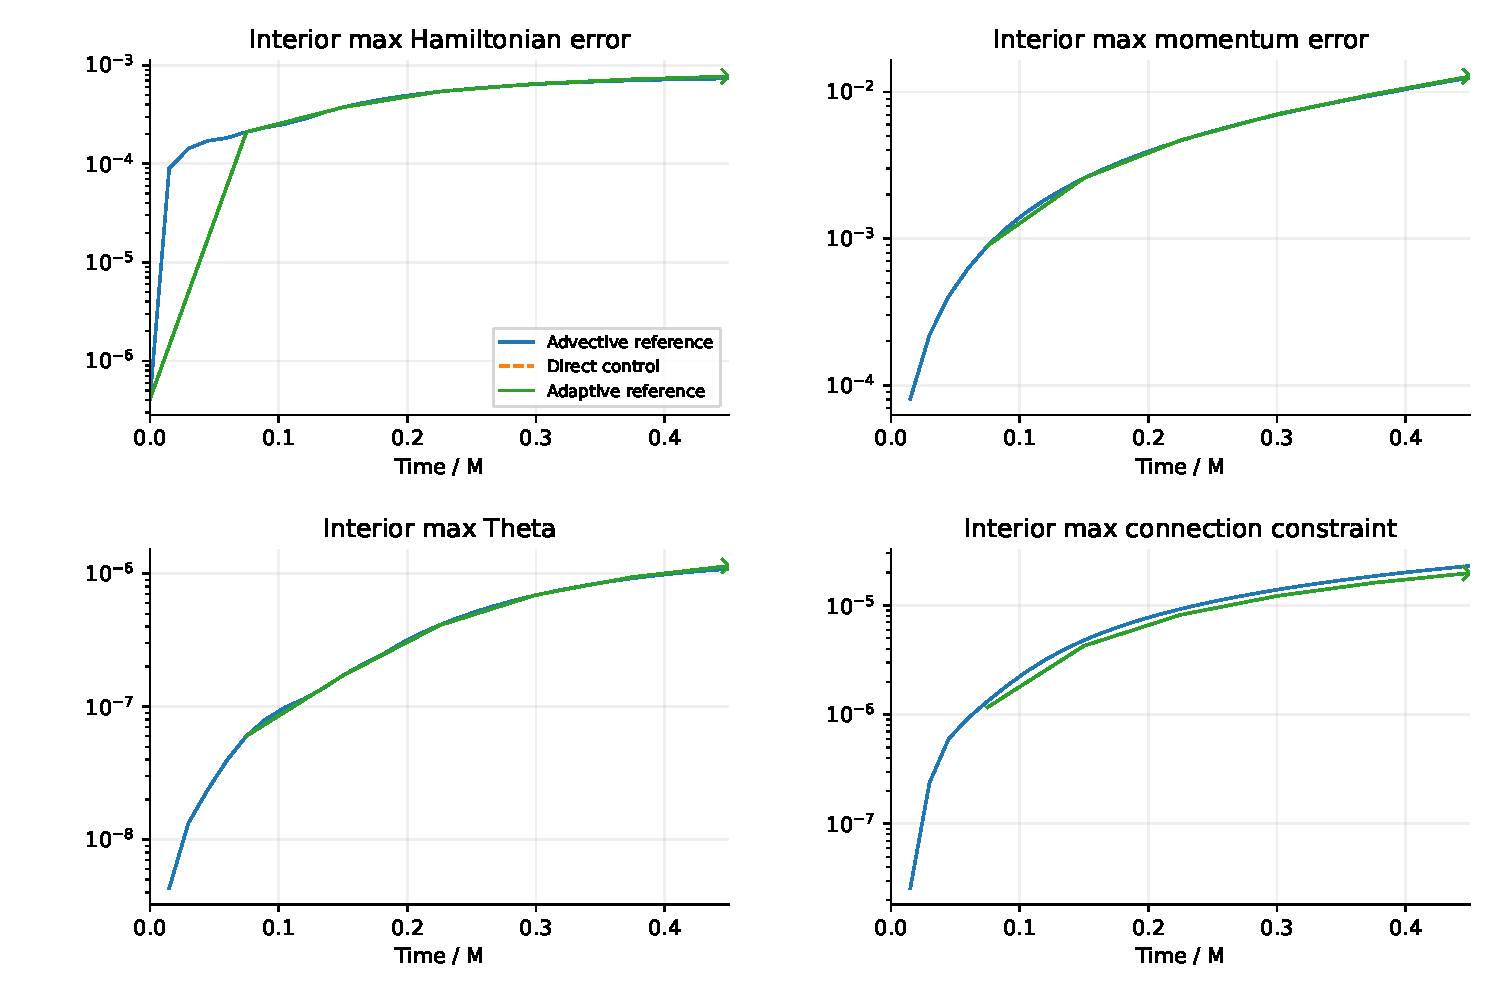
\includegraphics[width=\linewidth]{figures/interior-errors.pdf}

\caption{Interior constraint errors are retained separately and do not enter the exterior accuracy budget. No positive-radius neighborhood has been silently removed.}\end{figure}

\begin{figure}[htbp]\centering

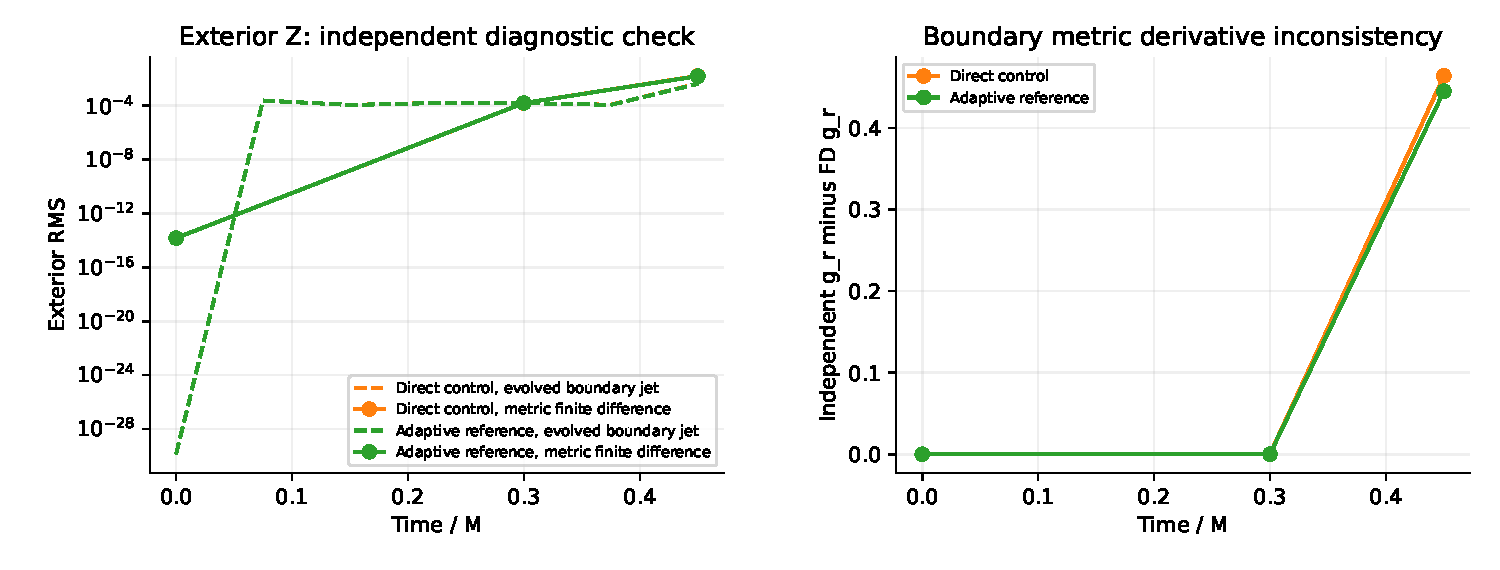
\includegraphics[width=\linewidth]{figures/constraint-definition.pdf}

\caption{The independent constraint-definition audit. Dashed curves use evolved boundary jets; solid markers reconstruct the derivative from metric values. Their difference exposes the reduction-consistency failure instead of suppressing its endpoint contribution.}\end{figure}

\begin{figure}[htbp]\centering

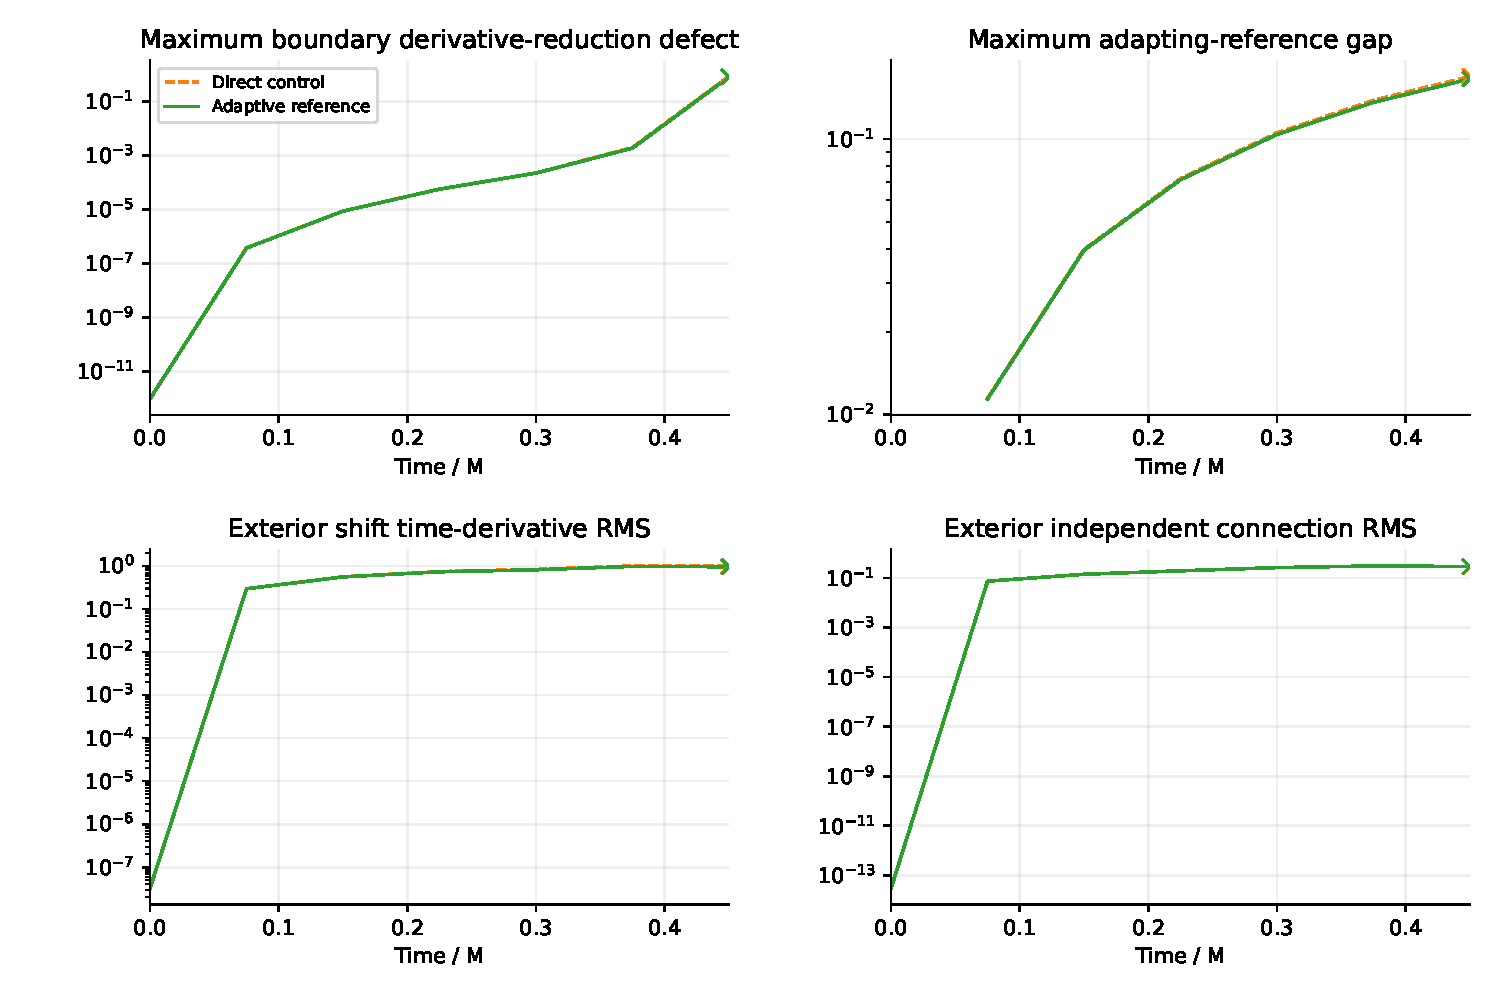
\includegraphics[width=\linewidth]{figures/reduction-and-settling.pdf}

\caption{Boundary derivative-reduction defects, reference gap, shift rate, and independent connection residual. These distinguish coordinate settling from simple horizon-radius flattening.}\end{figure}

\begin{figure}[htbp]\centering

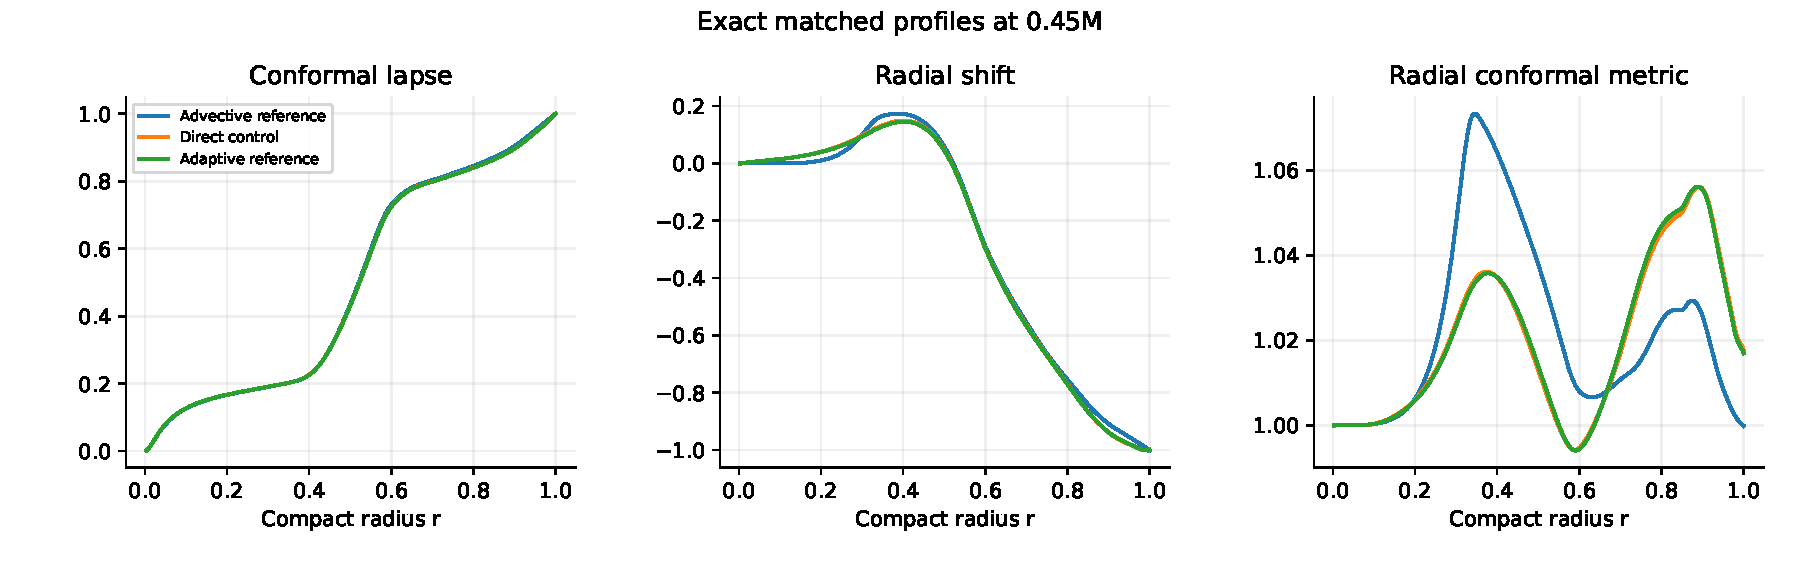
\includegraphics[width=\linewidth]{figures/matched-profiles.pdf}

\caption{Lapse, shift, and radial metric at an exact common saved time. Every positive-radius node is retained; the central coefficient endpoint is not a physical puncture sample.}\end{figure}

\FloatBarrier\subsection{Boundary timestep and diagnostic checks}

For the direct control at $N=33$, halving the timestep changes the dominant growth rate from 11.40269 to 11.40269 per unit coordinate time. The growing frozen mode therefore persists under this timestep reduction; the result is not explained by a large RK step alone.

For the adaptive control at $N=33$, halving the timestep changes the dominant growth rate from 10.86828 to 10.86828 per unit coordinate time. The growing frozen mode therefore persists under this timestep reduction; the result is not explained by a large RK step alone.

An independent recomputation of the native constraints replaces the evolved endpoint derivative reductions by ordinary finite-difference derivatives on every saved profile and last accepted state. Maximum changes in the H, M, Theta, and Z diagnostics are respectively $0,\ 0,\ 0,\ 2.278\times10^{-1}$. The Z difference is material and the metric-reconstructed Z norm is therefore used for the primary comparison. This exposes the boundary consistency failure; it does not repair the evolution.

\subsection{Answers to the comparison questions}

The tested implementation has no qualified $100M$ result. Reduced late-time horizon drift and competitive long-time exterior constraints or mass conservation are therefore unestablished. Exact nullness is assessed on the actual evaluated stages, not extrapolated to an unperformed long run. The numerical boundary growth prevents a claim of improved settling or robustness. No nearby reference-rate scan is justified by a failure already localized in the boundary discretization.
